\documentclass{article}
\usepackage{spconf}
\usepackage{amsmath}
\usepackage[dvips,pdftex]{graphicx}
\usepackage{subfigure}
\usepackage{named}
\usepackage[dvips,pdftex]{hyperref}
\title{Sketch Recognition using Particle Swarm Algorithms}
%\sthanks{Professor}\sthanks{Associate Professor}\sthanks{Professor}\sthanks{Associate Professor}
\twoauthors
  {Maha El Meseery, Mahmoud Fakhr El Din, Samia Mashali}
	{Signals Processing Group \\ Computers and Systems Department \\
  Electronic Research Institute\\Cairo, Egypt\\
	melmeseery@eri.sci.eg, samia@eri.sci.eg}
  {Magda Fayek, Nevin Darwish}
	{ Computer Engineering Department\\
	Faculty of Engineering \\Cairo University\\Cairo, Egypt\\
	magdafayek@gmail.com,ndarwish@ieee.org}
\begin{document}
\maketitle
\begin{abstract}
Sketch recognition is defined as the process of identifying symbols that users draw using single or multiple strokes. Users draw strokes using a pen and the system immediately interprets their strokes as objects that can be easily manipulated. This paper uses Particle Swarm Optimization Algorithm (PSO) to divide the strokes the user draws into meaningful geometric primitives. These geometric primitives are grouped to formulate symbols which are further identified. The results show that using PSO improves segmentation results which guide the symbol recognition phase. This paper uses Support Vector Machines (SVM) classifier which further improves the final recognition accuracy.  
\end{abstract}
\section{Introduction}
The field of symbol recognition has gained interest in the last few years. Scientists generally and engineers specifically express thoughts and designs using sketches. Engineers use sketches to exchange designs as a natural method of communication rather than writing or speaking. Design engineers need a powerful computer based system with symbol recognition to help them design, manipulate and store sketches more effectively than using only papers. Increasing the interaction between computers and users in sketch and CAD systems has been the reason for the emerging of a few advanced sketch recognition systems. Sketch recognition is the process of identifying user strokes into meaningful symbols that can be further used.  
%Sketch recognition is divided into three main steps preprocessing, segmentation and symbol recognition. The preprocessing phase captures user input stroke points and collects basic information about the stroke then proceeds to remove noise and compute basic statistical and geometrical information. In segmentation phase, the strokes are divided into a set of simple geometrical primitives or segments. In the third phase, sketch recognition, strokes and segments are clustered to formulate symbols that can be recognized by a classifier system. 

A wide variety of techniques were suggested for sketch recognition.  A hybrid algorithm was introduced in \cite{earlyprocess} where they generated different sets of segments based on both curvature and speed dominant points, followed by choosing a segmentation with the least error from a generated hybrid set. Their system is however limited to recognizing only specific simple geometric shapes with a set of low level recognizers. Each low level recognizer is designed to recognize only one geometric shape using spatial and geometric information extracted from the stroke.  Yu \cite{meanshift10} introduced a feature area for each primitive and then computed the segmentation error for different types of primitives based on the computed feature area. His system achieved good accuracy in simple shapes (square, ellipse,...) but did not perform well in more complex shapes. Paulson and Hammond\cite{Paleosketch08} introduced a set of low level recognizers that were reported to achieve 98\%  accuracy but their system, similar to all low level recognizers, only identify a small set of simple shapes. One of the problems in these previous systems is that they only rely on curvature and speed data which are subjected to noise. They are also subjected to over and under segmentation problems due to use of thresholds. 

The segmentation problem is summarized as finding the best decomposition with least number of segments each represents a geometric primitive. This is an optimization problem, which evolutionary programming can solve efficiently. A genetic algorithm was used by \cite{CruveDivisionSwarm} to optimally divide digital curves into lines and curves. Chen et al.\cite{CruveDivisionSwarm} uses digital curves scanned from paper as input to the system and did not take advantage of the curvature or local geometric properties of the digital curve.

This paper introduces a new sketch recognition system, which uses particle swarm algorithm (PSO) to optimally segment user's strokes. Users can draw symbols using any number of strokes in any order they like. The system segments each stroke using two different PSO algorithms. Segmentation is based on dividing the digital curve into polygon\cite{PolygonApproximationPSO}. To handle complex strokes, our system uses a second segmentation PSO algorithm to segment strokes into a set of lines and circular arcs. After segmentation, a symbol features vector composed of different statistical, geometrical and spatial features is deduced. The final classification step, SVM classifier uses the computed feature vector to classify the segments into one of the previously trained classes. 

The contribution in the system is mainly in attempting to generate the optimal segmentation using PSO which exhibited superiority with respect to similar algorithms in various other applications \cite{PolygonApproximationPSO}. The system attempts to find the optimal decomposition of the input stroke using PSO with the help of curvature and speed information. The use of PSO algorithm helps in eliminating the effects of input noise, problems of over and under segmentation that were in pervious systems. The proposed symbol recognizer uses the generated segmentation to compute the feature vector which is used to identify more complex symbols. This enables the system to be scalable for more complex shapes. 

 %The remaining of the paper is as following; Section \ref{Sysdisc} describes the system in details. Sections \ref{Prepross}, \ref{seg} and \ref{sec:Recognition} provide details on preprocessing, segmentation and recognition process respectively. Section \ref{sec:Experiments} describes the experiments that were preformed. We conclude in Section \ref{ConclusionandFutureWork}.
 
\section{The proposed system}
\label{Sysdisc}
 The suggested sketch recognitions system is divided into three main steps 1) preprocessing, 2) segmentation and 3) Recognition. The following section provides a detailed description of each step.
\subsection{Preprocessing}
\label{Prepross}
 Speed and time difference information were widely used in sketch understanding systems \cite{earlyprocess}. It was noted that time difference provides more distinct maxima than the speed information. Agar \cite{polygonfeedback31} mentions that the pointing device (i.e. the mouse) sampling rate is the reason for this phenomenon. 
 In the presented system, we computed time difference, direction, speed and curvature of each point along a stroke. The speed is calculated as $v=\Delta s/\Delta t$ where $t$ is the time difference between two points and $s$ is the length between them. The direction $d$ is calculated as the angle between two vectors and curvature is considered as the change in direction with respect to length i.e. $c= \Delta d/\Delta s$. Dominant points are characterized by lower speed values and higher curvature and direction values.
  
After the system computes all the speed, time difference and curvature information it proceeds to detect the points with low velocity and high curvatures. Using simple differentiation to detect local extreme points resulted in false points due to the non smooth curves. Hence, the system adopted a process presented by \cite{earlyprocess}, where the mean of the curve is calculated. Then a threshold \textit{th} is used to separate the curve into regions $Region_i$; each region $Region_i$ is defined as a range of points, where the curve values are either above or below the threshold \textit{th}. Those regions are further processed to find the maximum point $Max(Region_i)$ of each region $Region_i$. The stroke points $p_i(x,y)$ that correspond to those maximum values are labeled as \textit{possible dominant points} $P_{pd}$. The system repeats this process for curvature, time difference and speed information. All the points labeled as possible dominant points $P_{pd}$ are saved into a single array. Figure \ref{fig:LabelsPPD} shows the particles labeled as Possible dominant point $P_{pd}$ by the preprocessing, it is noticed the redundancy of some $P_{pd}$ points. % (as shown are redundant)
\begin{figure}
	\centering
		\subfigure[Posible domninate point]{ 	
		\label{fig:LabelsPPD}	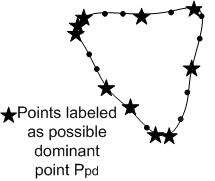
\includegraphics[scale=0.5]{images/ppd.jpg}}
		\hfill
			\subfigure[DPSO algorithm encoding]{	
			\label{fig:LabelsPSO} 
			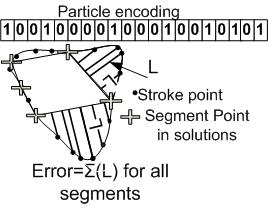
\includegraphics[scale=0.5]{images/pso1.jpg}}			
	\caption{Segmentation}% a) Possible dominate point b) Particle encoding  
	\label{fig:pso1}
\end{figure}
\subsection{Segmentation}
\label{seg}
In the segmentation stage the stroke is divided into a set of primitives. As shown in Figure \ref{fig:segblock} first an attempt is made to fit the stroke points into a curve or an ellipse using a minimum square error fitting algorithm. If the stroke proved to be an ellipse arc then the segmentation process ends and the system proceeds to the next step. Otherwise, the stroke is passed to two particle swarm algorithms that divide the stroke to either lines or lines and curves. The algorithms takes the stroke points along with the possible dominant points $P_{pd}$ computed during preprocessing then produce a set of dominant points which are connected by either lines or curves.  The next section describes the ellipse detection algorithm and the two particle swarm algorithms used to divide the stroke.
 \begin{figure}
	\centering
		\includegraphics[scale=0.55]{images/segblock.jpg}
	\caption{Segmentation Block}
	\label{fig:segblock}
\end{figure}
\subsubsection{Ellipse Detection} 
The process starts by computing the center of the stroke bounding box. The bounding box center point is used as the first estimation of the ellipse center. The axes of the ellipse are estimated as $width/2$ and $height/2$ of the stroke bounding box. The least square fitting algorithm is used to minimize the fitting error of the ellipse equation.  

\subsubsection{Discrete particle swarm algorithm (\textit{DPSO})}
\label{subsubsec:Discreteparticleswarmalgorithm}
Two DPSO algorithms are used to generate segmentations for each stroke the user draws. For each generated segmentation an error is determined. The segmentation with the minimum error value is chosen as the best stroke segmentation (Figure \ref{fig:segblock}). The problem definition is the same in both algorithms but they differ in the method they use to compute fitness and error functions \footnote{The parameters of the DPSO algorithms are determined using empirical experiments and conform with similar applications \cite{PolygonApproximationPSO} (e.g. 15 particles, 80 maximimum swarm iteration)}. 

\textsl{Problem definition:} The input stroke with $N$ points can be represented by set $S = \left\{ {x_1 ,x_2  \ldots x_N }\right\}$ where $x_i$ is the location of the point $i$. The swarm algorithms consist of $M$ agents which are represented by the set  $A = \left\{ {P_i \left| {i = 1,2 \cdots M} \right.} \right\}$ where $P_i$ is a single solution particle from the solution space. Each particle decodes the problem using a binary array with the same length $N$ as the input stroke.  

Therefore, the system represents each particle $P_i$ by $P_i = \left\{ {p_{ij} \left| {j = 1,2 \cdots N} \right.} \right\}$ where $p_{ij}$ has only two values 0 or 1. $p_{ij}=1$ means that point $j$ is a dominant point. Figure\ref{fig:LabelsPSO} shows a particle encoding in the DPSO system. 

\textsl{Fitness function:} The fitness function and error calculation are different in each of the two \textit{DPSO} algorithms. 

For the \textit{first algorithm \textsl{AlgS1}}, the arc $\widehat{x_lx_k}$ is defined as the consecutive set of points from point$x_l$ to point $x_{k}$ as in $x_l,x_{l+1} \cdots,x_k$. The line $\overline{x_l x_k} $ as the straight line connecting point $x_l$ to point $x_k$. The approximation error is computed by the equation \ref{eq:ErrorSwarm1}. The graphical meaning of the error is shown in Figure\ref{fig:LabelsPSO}.
\small \begin{equation}
E=\sum\nolimits_{l = 1}^M e ( \widehat{x_lx_{l+1}},\overline{x_l x_{l+1}})
\label{eq:ErrorSwarm1}
\end{equation} 
\normalsize
where $M$ is the number of dominant points in this solution as generated by the swarm algorithm. The error $e ( \widehat{x_lx_k},\overline{x_l x_k})$ is computed as the sum of squared perpendicular distance from every point along the arc $\widehat{x_lx_k}$ to the line $\overline{x_l x_k}$. The fitness is computed using equation \ref{eq:fitnessSwarm1}
\small \begin{equation}
\max fitness(p_i ) = \left\{ {\begin{array}{*{20}c}
   { - E/\varepsilon N} & {ifE > \varepsilon ,}  \\
   {D/\sum\limits_{j = 1}^N {p_{ij} } } & {otherwise}  \\
\end{array}} \right.
\label{eq:fitnessSwarm1}
\end{equation}\normalsize where $N$ is the number of points in the stroke, $D$ is the number of points in the solution that was previously labeled as a possible dominant point ($P_{pd}$), $E$ is the computed error and $\varepsilon$ is the error threshold. It should be noticed that when the error is larger than the threshold $\varepsilon$ the fitness is given a $-ve$ value to lower the fitness value of the solution. Otherwise the system favors the lower number of vertices.

The previous algorithm segments stroke into set of line segments but strokes does not always consist of line only. It is more meaningful to use curves when segmenting strokes. Therefor, a \textit{second algorithm \textsl{AlgS2}} is used to decompose strokes to set of lines and circular arcs. \textit{\textsl{AlgS2}} has the same problem formulation but different fitness and error functions are used. An attempt is made to fit each segment into line or circular arc, the error of both circle and line fit estimations are computed for each segment $S_s=\widehat{x_lx_k}$, the approximation with the lower error value is the chosen approximation of this segment $S_s$\cite{CruveDivisionSwarm}. The sum of the approximation error of all segments is the total error of the particle. The total error of the particle is computed by equation \ref{eq:errorSwarm2}
\small \begin{equation}
E=\sum\nolimits_{s = 1}^M e(D_s) 
\label{eq:errorSwarm2}
\end{equation} \normalsize where $M$ is the number of segments in the solution as generated by the swarm algorithm, $D_s$ is the minimum approximation error of curve and line approximations $min(d_c,d_l)$ as computed by \cite{CruveDivisionSwarm}.  The fitness is computed by the equation \ref{eq:fitnessSwarm2} \small \begin{equation}
\max fitness(P_i ) = \frac{1}{{E \times M^k }}
\label{eq:fitnessSwarm2}
\end{equation} \normalsize where $E$ is the error and $M$ is the number of segments and $k$ is a parameter tweaked to get minimum number of segments. The larger $k$ is, the more effect the number of segments will have. For our system, $k$ is selected to be $0.5$\cite{CruveDivisionSwarm}.

After each loop of the swarm algorithm (\textsl{AlgS1} and \textsl{AlgS2}), each particle is refined using the following procedure. For each particle $P_i$ each dominant point $P_{ij}$ is checked to find if it was labeled before as a \textit{possible dominant point} $P_{pd}$ (computed as in section \ref{Prepross}). If it was not labeled the point $P_{ij}$ is moved to the nearest labeled point. This ensures that all of the points generated by the DPSO are possible dominate points $P_{pd}$. After that the particles are tested to make sure that the distance between every two successive dominate point is larger than the constant $min_D$. If two points are nearer than $min_D$ then one of the points is removed. 
\subsection{Recognition}
\label{sec:Recognition}
After the user draws all strokes of the symbol, the set of un-recognized strokes is grouped together along with their segmentation as input to the feature extraction process. A composite set of features is used to generate a single feature vector. The features used consist of Rubine feature set,  Zernike moments of order 10 \cite{HeloiseBeautification}, ink density as well as some structural and spatial information like number of perpendiculars lines ,number of parallel lines and number of different types of primitives in each symbol. After computing the features the symbol is introduced to the (SVM) classifier. 
\section{Experimental}
\label{sec:Experiments}
 
The dataset collected by Hse and Newton\cite{HeloiseBeautification} is used to test the presented system.  Figure \ref{fig:symbolSet} shows a set of the shapes used in the data set. The datasets were divided into training and test sets. Five different splits for the training and test data are generated from each dataset. The results displayed are the average recognition accuracy of the five splits. The accuracy is computed as the number of correctly recognized samples divided by the total number of samples in the test.
 \begin{figure*}[]
	\centering
	\begin{minipage}[b]{5cm}	
\begin{center}
\subfigure [The Symbol Set] {\label{fig:symbolSet}
\fbox{ \parbox{2cm}{% 
		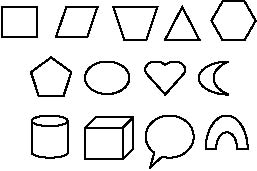
\includegraphics[scale=0.2]{images/symbolSet.PNG}	}}}
		
		\subfigure[Algorithm comparison]{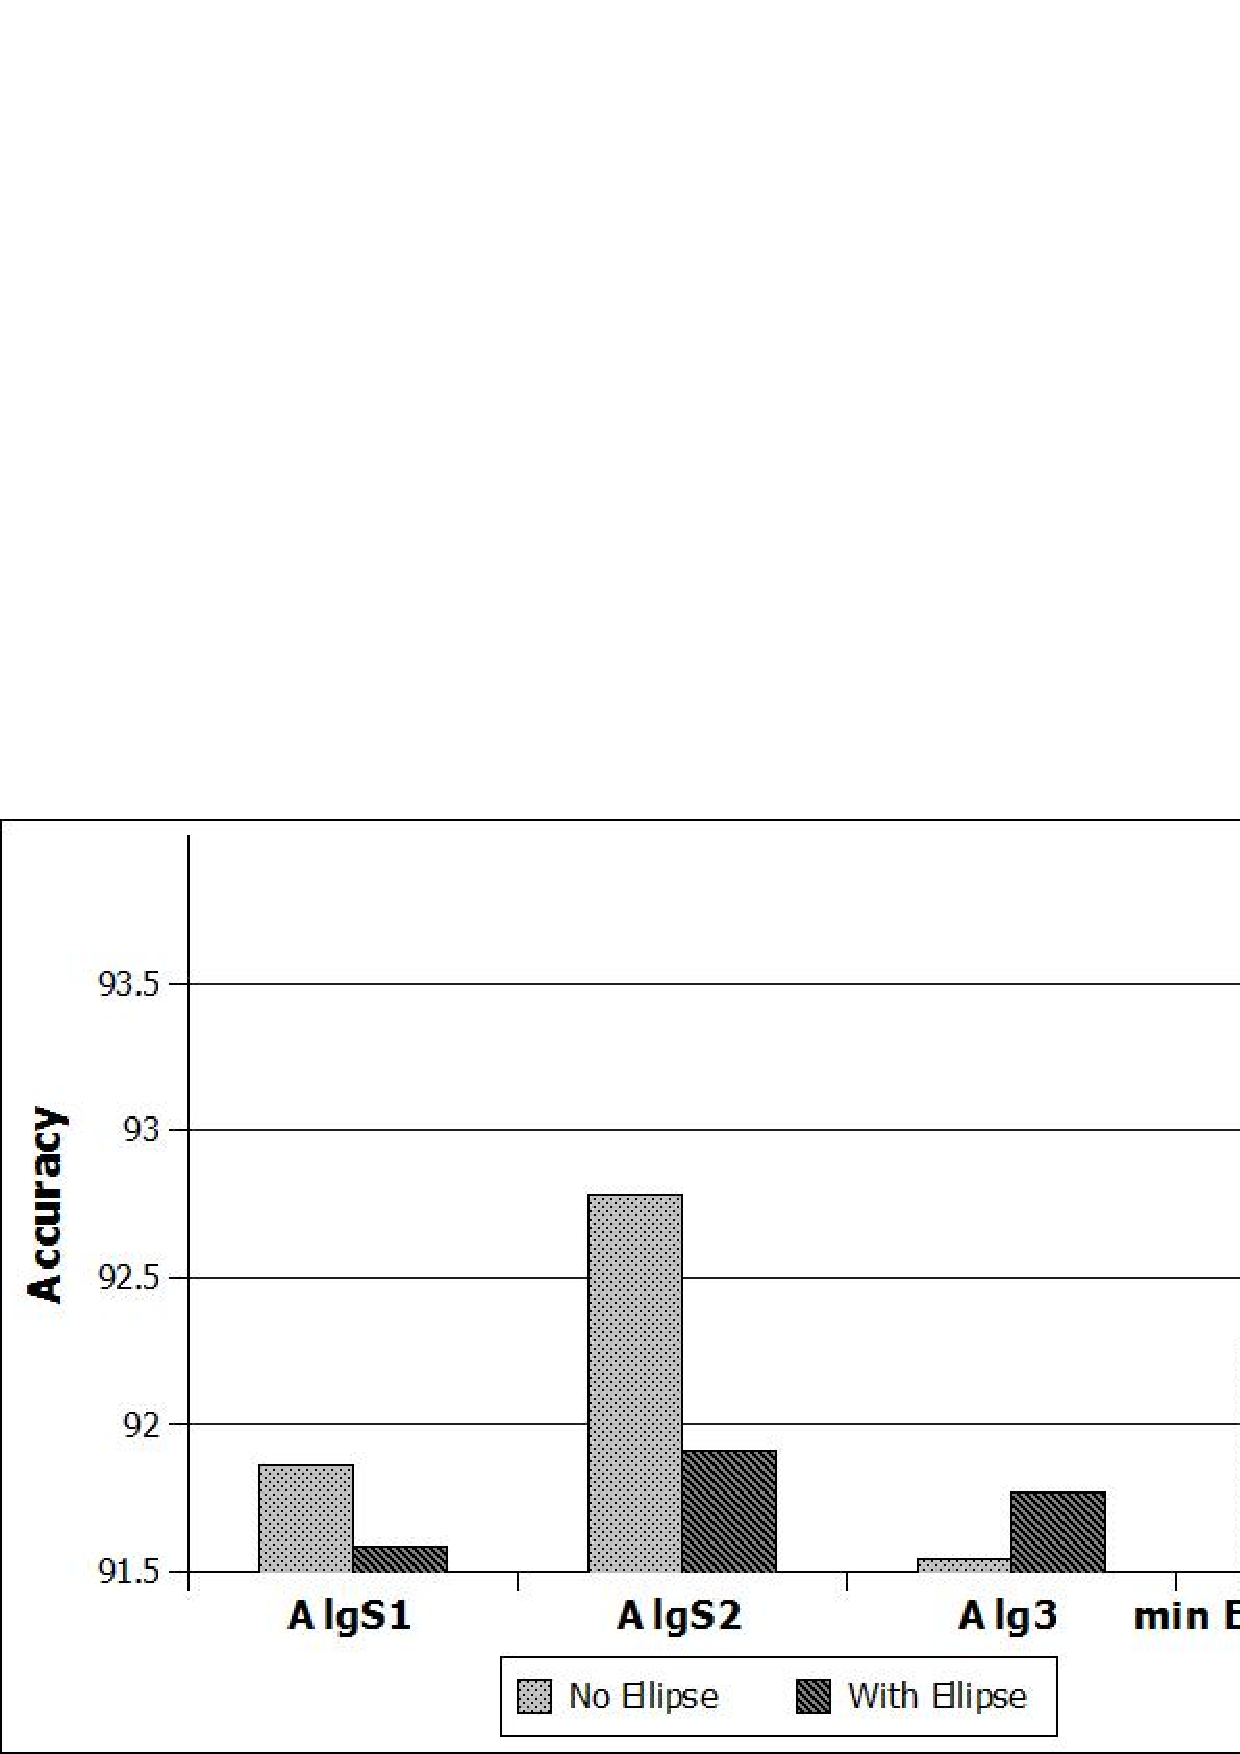
\includegraphics[width=5cm]{images/testAlg.jpg} 	\label{fig:test1}}
		\end{center}
		\end{minipage}
		\hfill
  \subfigure [Symbols Comparison] {\includegraphics[width=11cm]{images/symbols.jpg} \label{fig:test2}} %symbols.jpg  test2smallpaper.jpg
	\caption{Experiments results :} a) The symbols set used in the dataset.   b) The recognition rate of different algorithms.  c) The recognition rate of each symbol using different algorithms. 
\end{figure*} 
We performed two experiments to test the system. Firstly, we tested recognition accuracy of shapes in the data set with both algorithms (\textsl{AlgS1} and \textsl{AlgS2}). We also implemented the segmentation algorithm described in \cite{earlyprocess} (\textsl{Alg3}) to compare it with our swarm algorithms. Figure \ref{fig:test1} shows the accuracy achieved by each algorithm. The result shows that (\textsl{AlgS2}) gives better performance than Alg3 and AlgS1. 
% Firstly we tested recognition accuracy of shapes in the data set with both algorithms (\textsl{AlgS1} and \textsl{AlgS2}). Figure \ref{fig:test1} shows the accuracy achieved by each algorithm. The two swarm algorithms were tested with and without the ellipse fitting module. Including the ellipse detection module improves the results with both the \textit{DPSO} algorithms.% The results show that both \textit{DPSO} algorithms achieve better result than other algorithms. The two swarm algorithms were tested with and without the ellipse fitting module. Combining the ellipse detection module improves the performance in the tested dataset.  

The second experiment we implemented was to test the effect of symbol complexity and type on the recognition rate. Figure \ref{fig:test2} shows the accuracy of each symbol, it is clearly noted that symbols that have only line segments achieve higher accuracy rate than other symbols. Figure \ref{fig:test2} also indicates that algorithm \textsl{AlgS1} alone achieve better performance than algorithm \textsl{AlgS2} in the symbols that consist only of lines. This is natural as algorithm \textsl{AlgS1} divides strokes into line segments only but \textsl{AlgS2} is able to divide strokes into lines and curves based on the minimum error of the segment itself. Combining both algorithm \textsl{AlgS1} and \textsl{AlgS2} improved the recognition rate of all symbols. The penalty for this increased performance is in the computational time needed to run both swarm algorithms. 
 
\section{Conclusion and Future Work}
\label{ConclusionandFutureWork}
This paper presented a new approach to sketch recognition using DPSO. Results show that the \textit{DPSO} in general generates an optimized stroke segmentation which improves the final recognition rate.  The final recognition is based on geometrical, statistical and structural features. The experiments evaluated two \textit{DPSO} different segmentation algorithms (AlgS1 and AlgS2) on simple presentation set dataset. Results show that AlgS2 achieves better segmentation and final accuracy than Alg3 \cite{earlyprocess} on the dataset used. The results proved that the system is easily expandable to more and more symbol as it does not depend on low level primitive recognizers but on high level symbol and geometrical features.  The system achieved an average overall improvement of more than 2\% over Alg3.  
%This paper presented a new approach to sketch recognition using PSO. The system uses both speed and curvature information which help improving the \textit{DPSO}. It is noted that the \textit{DPSO} in general generates an optimized stroke segmentation which improves the final recognition rate.  The tradeoff between accuracy achieved and time complexity must be further investigated to achieve better results. The use of statistical moments and structural features improves the recognition rate. The system was tested on 13 different symbols and achieved an accuracy of 91.5\%. The system does not depend on low level recognizer but rather on a set of high level features. This makes the system easily expandable to more and more symbols. 

 A possible extension of this research is to complete the clustering algorithm for fully automated sketch recognition. Currently, the system process one symbol at a time, an enchantment would be to allow users to draw more than one symbol at a time and incorporate a method for separating symbols. Other area of enhancements is the features extraction methods. Introducing more spatial and geometrical features is believed to improve classifications.  
 
\bibliographystyle{IEEEbib}
\bibliography{../../neededfiles/Bibliographies/Mybibliography}
\end{document}
